\documentclass[11pt]{article}
\usepackage{fontspec}
\usepackage{hyperref}
\usepackage{graphicx}

\newcommand{\OC}{\textsc{Ococo}}
\newcommand{\AC}{Ad hoc script}

\begin{document}


\section*{Supporting Information -- S1 file}
\subsection*{\emph{K. Břinda, V. Boeva, G. Kucherov: Dynamic read mapping and online consensus calling for better variant detection}}


To evaluate different read mapping scenarios with Dynamic Mapping Simulator (\url{http://github.com/karel-brinda/dymas}),
we designed a series of runs (Table~\ref{tab:all_runs}) with several different parameters (Table~\ref{tab:options}). For all experiments described in the paper, all runs were performed. In our analysis, we mainly considered several selected runs, which we compared in a particular way (Figure~\ref{fig:selected_runs}).

Generated PDF reports for all runs can be found in \textbf{S2 file}. Full HTML reports (files \texttt{3\_evaluation.html}) for all runs are located in git repository
\url{https://github.com/karel-brinda/dymas} in directory \texttt{experiments}. For instance, subdirectory \texttt{exp2.01\_\_Tuberculosis\_\_0.07-baq} corresponds to Experiment~2, Run~01.


\clearpage

%%%%%%%%%%%%%%%%%%%%%%%%%%%%%%%%%%
\begin{table}[h!]
\begin{center}
\begin{tabular}{lll}
        \textbf{Run} & \textbf{Mutation rate} & \textbf{Options}\\\hline
        x.01 & 0.07 & baq \\
        x.02 & 0.07 & \\
        x.03 & 0.07 & ococo32 \\
        x.04 & 0.07 & ococo16 \\
        x.05 & 0.07 & delstats \\
        x.06 & 0.07 & ins, dels \\
        x.07 & 0.07 & delstats, baq \\
        x.08 & 0.07 & dels \\
        x.09 & 0.07 & bowtie2 \\
        x.10 & 0.07 & ins \\
        x.11 & 0.07 & ococo16, noremap \\
        x.12 & 0.11 & \\
        x.13 & 0.13 & \\
        x.14 & 0.15 & \\
        x.15 & 0.07 & delta500 \\
        x.16 & 0.07 & bowtie2local \\
        x.17 & 0.07 & ococo16, stochastic
\end{tabular}
\end{center}
\caption{List of all runs with their assigned options.}
\label{tab:all_runs}
\end{table}
%%%%%%%%%%%%%%%%%%%%%%%%%%%%%%%%%%

\clearpage


%%%%%%%%%%%%%%%%%%%%%%%%%%%%%%%%%%
\begin{table}[h!]
\begin{center}
\begin{tabular}{lp{3cm}p{9cm}}
\hline\\
\textbf{Option} & \textbf{Simulation} & \textbf{Description} \\
\\
\hline
\\
\textbf{BAQ} & \AC &
        Allow base alignment quality recalibration in \texttt{samtools mpileup} (otherwise called with the \texttt{--no-BAQ} option). 
        \\ \\
\textbf{DelStats} & \AC &
        Add number of deletions to coverage (with coverage derived from A, C, G, T counters only, decision about updates with the majority strategy at a position with many deletions may be incorrect).
        \\ \\
\textbf{Bowtie2} & \AC &
        Use Bowtie~2 in the global mode for read mapping instead of BWA-MEM.
        \\ \\
\textbf{Bowtie2local} & \AC &
        Use Bowtie~2 in the local mode (option \texttt{--local}) for read mapping instead of BWA-MEM.
        \\ \\
\textbf{Delta500} & \AC &
        In evaluation using RNFtools, set \texttt{allowed\_delta} (tolerance, see \url{http://rnftools.readthedocs.io/en/latest/reference/02_lavender.html}) to 500.
        \\ \\
\textbf{Ococo} & \OC &
        Call consensus with \OC~(with statistics of $16$ or $32$ bits per position, i.e, using $3$ or $7$ bit counters, respectively) instead of \AC.
        \\ \\
\textbf{NoRemap} & \OC &
        Do not simulate remapping.
        \\ \\
\textbf{Ins} & \OC &
        Allow insertion updates.
        \\ \\
\textbf{Dels} & \OC &
        Allow deletion updates.
        \\ \\
\textbf{Stochastic} & \OC &
        Use the stochastic strategy in \OC~(parameter \texttt{--strategy stochastic}) instead of the majority strategy.
        \\ \\
\end{tabular}
\end{center}
        \caption{
                Possible options for a run.
        }
        \label{tab:options}
\end{table}
%%%%%%%%%%%%%%%%%%%%%%%%%%%%%%%%%%

\clearpage

%%%%%%%%%%%%%%%%%%%%%%%%%%%%%%%%%%
\begin{figure}[h!]
        \begin{center}
        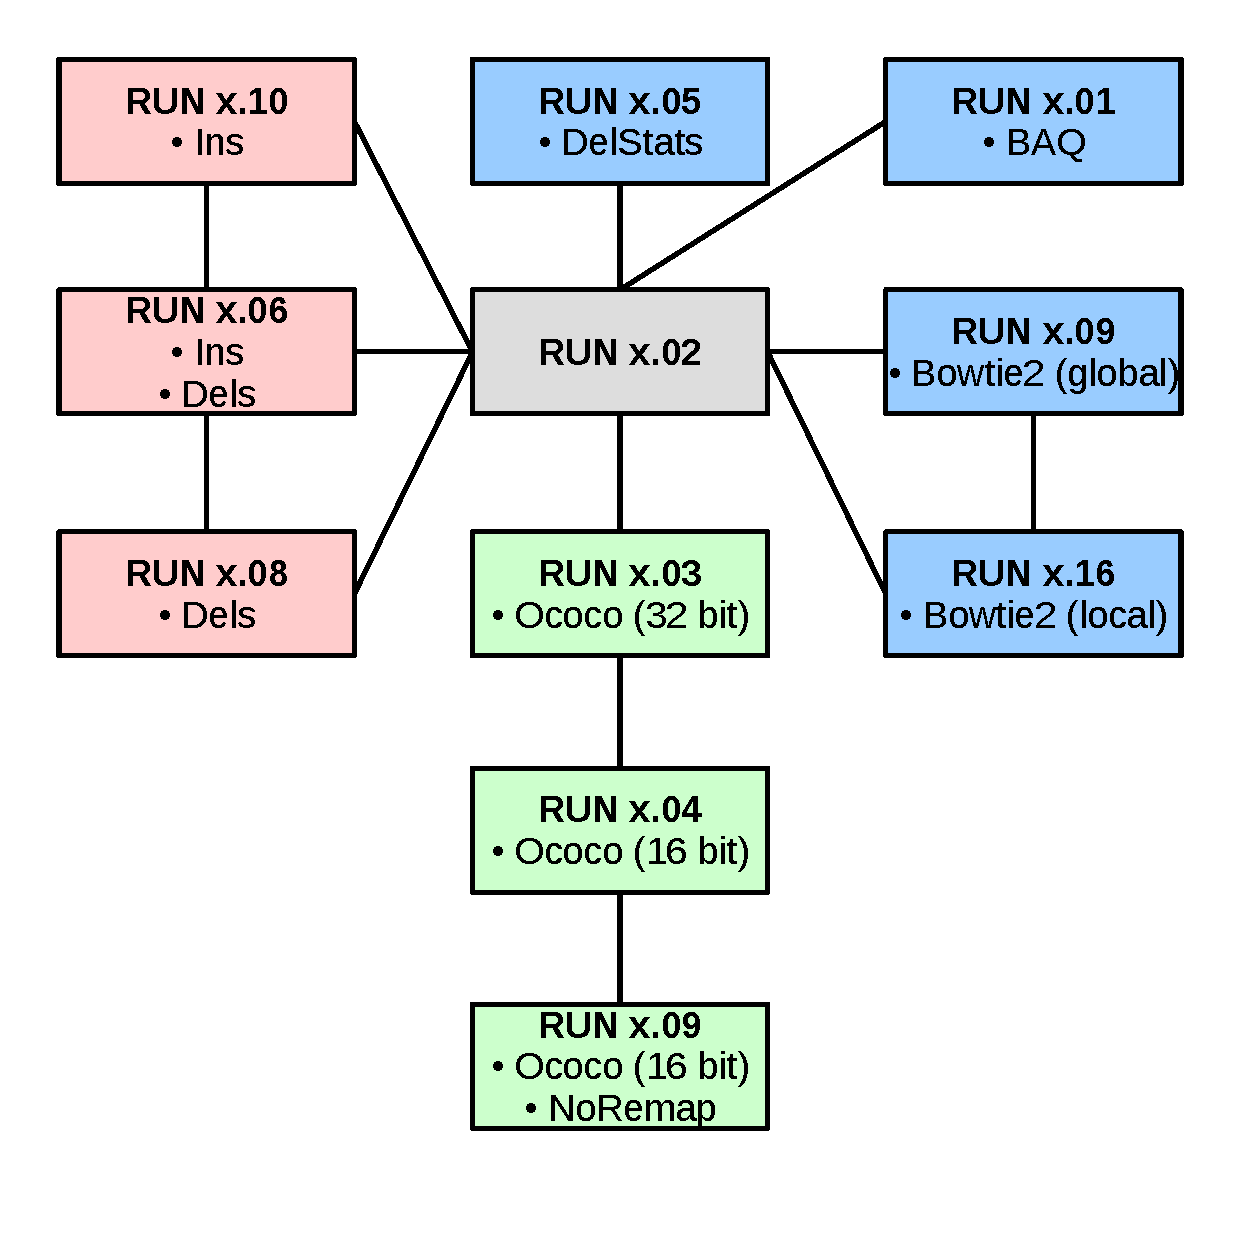
\includegraphics[width=8cm]{runs_scheme.pdf}
        \end{center}

        \caption{
                Scheme of selected runs with their options. Edges signalize runs to be considered for a mutual comparison.
        }
        \label{fig:selected_runs}
\end{figure}
%%%%%%%%%%%%%%%%%%%%%%%%%%%%%%%%%%




\end{document}
